\section{Huge Pages}
	\label{sec:hugepage}
Huge pages are an optimization with the demand of high performance. On latest
Intel x86-64 platform, the page size can be even 1GB. This provides good
chance for those applications suffer from virtual memory abstraction to tune
their performance, like the databases, or the host mode virtual machine monitors.
The benefits of huge pages have been long mentioned, but viewing from the
virtual memory system, there could be very time consuming to prepare these
huge pages, since huge page means continuous in physical, and it will be very
difficult to find out large chunks of physical continuous spaces if the system is
at busy time. In this section, I try to measure the cost to use huge pages.

\subsection{Methodology}
The experiments will contain two part, the first is the time to prepare huge
pages. This would be carried out after a busy period to observe the effect. I
choose to measure this after each Interval of section~\ref{sec:sharedobj}. Then
I try to illustrate the different timing behavior when using large pages and
small pages, by allocating the same amount of memory, and do several kinds of
walking on that.

Based on the experiments in section~\ref{sec:alloc}, it's obvious that if we
just reference a few bytes after requesting a huge page, the cost would be
larger than using a set of small pages. But this is meaningless in real
applications. So I use both sequential walking, and random access to test
the visiting time. Also, to justify the possible impact of allocation, I
also make walking happen several times: in real applications, it is not
strange to walk through a data area for several times, and the first time
page faults can be amortized in later walk.

\subsection{Experiments}
The first thing I tried to measure is the preparation time of the huge pages.
But it is quite fast on my machine, less than 1 second to prepare 5000 huge
pages. The workload I used to stress the system is mentioned in section~\ref{sec:alloc}. After each 5 run of the allocator testing, I checked the preparation time

\begin{figure}[hbt]
\centering
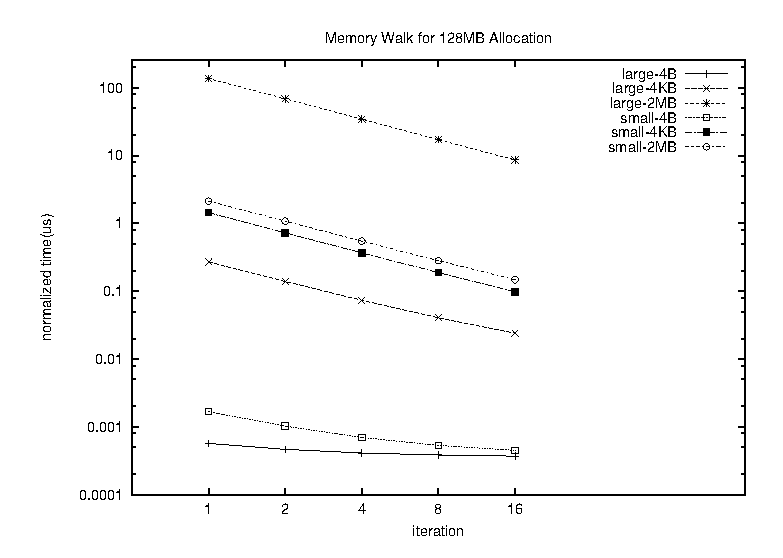
\includegraphics[width=0.9\linewidth]{../figures/hugetlb_128m}
\caption{Memory walk time on 128MB mapped memory. I use different stride, and
iterations for each walk, and measure the average time cost. The larger the 
stride size is, the worse performance I will get by using huge pages. Due to
space limitation, I didn't draw more stride result. Actually the small page
beats huge ones at the point of 32KB stride.}
\label{fig:hugetlb-time}
\end{figure}
\begin{figure}[h]
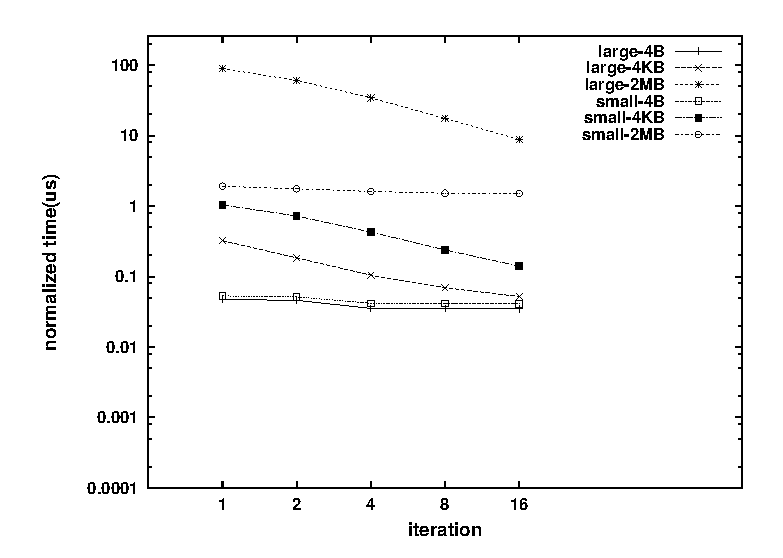
\includegraphics[width=0.9\linewidth]{../figures/hugetlb_rand_128m}
\caption{Random walking is similar with sequential walking, when in small stride
size the huge pages perform better. Here the stride is just used to determine the 
amount of memory reference, rather than walk pattern. I use stride to label it
just for comparison with sequential walk. One thing changes in random walk is
that for 4B stride, both of the two configurations perform worse than
sequential walk. The reason may be related with locality, but it is not what we
address here.}
\label{fig:hugetlb-rand}
\end{figure}

Figure~\ref{fig:hugetlb-time} shows the cost of walking on newly allocated
small and huge pages, total memory size is 128MB. The stride we used to walk on
the pages are from 4B to 2MB, with multiple iterations in each walk. It is quite
clear that huge pages performs bad when iteration number is small, and stride
is large. With the iteration increases, its average performance is
more improved.

Random walking shows similar trend as in figure~\ref{fig:hugetlb-rand}. Small
pages still perform better at the beginning, but normalized difference is
smaller. The result again illustrates the benefit of on demand allocation:
sequential walking will force all pages being brought into the systems, and
that may not be a must.

\subsection{Discussion}
Huge pages can be useful, especially when used by VMM, if no huge pages are 
used, then on a 4 level paging system, a page fault can visit memory up to 20 times 
to get a value. With the huge pages, this can be reduced to minimum. The problem
for the huge page is that it must be requested and configured explicitly, thus
 may lead to the memory pressure if used abusively. Another thing is the cognition
 of the cost of huge pages: for large data not frequently referenced, using 
 large pages may not get benefits.

Another thing strange is about requesting the pages, in Linux normal users can
get huge page through \emph{mmap} interface using anonymous mapping, without
causing protection problem.  However, the similar access through \emph{shmget}
interface will not work, unless super user privilege is granted. I didn't see
difference between this two approaches, hopefully it is not a security hole.
